\section{Introduction}

Bacterial biofilms are microscopic depositions of organisms that attach themselves on immersed surfaces whenever environmental conditions can sustain microbial growth.
These bacteria, when sessile, surround themselves in a self-produced viscous layer of extracellular polymeric substances.
As a result of this, the cells are extraordinarily resistant to mechanical washout or antibiotic attacks.
Most bacterial populations live in communities within the extracellular polymeric substances.
They can be found in many different aspects of life in both positive ways (wastewater treatments, soil remediation, and groundwater protection) and negative ways (bacterial infections, dental plaque, biocorrosion of facilities and water pipes).

The first biofilm models, like that in \cite{rittmann1980model}, assumed that biofilms developed as a flat layer and were posed as ordinary differential equations or one-dimensional partial differential equations.
This simplified the calculation for the speed of propagation but was limited in non-spatially heterogenous biofilm morphologies. %!% Source of an old paper would suffice
To this end, many models for spatially heterogenous biofilms were proposed.
These included stochastic individual based models \citep{kreft2001individual}, cellular automata models \citep{picioreanu1998newCombined}, and deterministic continuum models \citep{eberl2001deterministic}. 
The added complexity helped in modelling more of the multi-dimensional aspects of biofilms, namely the intrinsic structures that most biofilms grew.
These models considered the changes the biofilms made at the meso-scale instead of the reactor-scale which simpler models tended to do.

The recent field of energy biotechonology has led to researching biofilms as a potential means of using plant biomass to generate sustainable fuels. 
These fuels, such as ethanol, are generated through conversion of terrestrial or aquatic biomass \citep{lynd2008energy}.
The main benefits for using these fuel sources is that they produce much less greenhouse gases as seen in Figure \ref{fig:emissions}.
Using cellulolytic biofilms (cellulose degrading biofilms) to produce biofuels means that only non-edible cellulose is utilized instead of edible plants like corn.
%OLD Using cellulolytic biofilms as a source of biofuel means that the crop leftover, cellulose, is utilized so that no edible goods are used like with corn ethanol production.
\textit{Clostridium thermocellum} is a possible choice for achieving large scale biomass conversion. %!% according to who?
Because of this there has been a surge of studies based around its behaviours and characteristics.
An interesting feature of \textit{C.thermocellum} is that is grows as a thin cellulolytic monolayer and does not produce any extracellular polymeric matrix \citep{dumitrache2013formFunction}.
This is a stark contrast to typical biofilms which are notorious for forming complex mushroom or pillar shaped morphologies.

\begin{figure}[!htp]
  \centering
  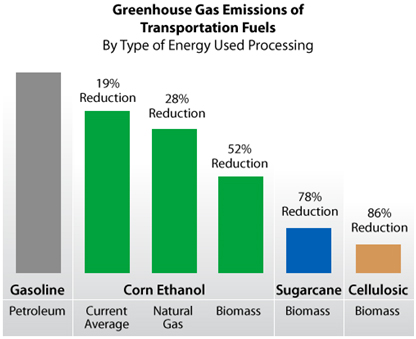
\includegraphics[scale=0.8]{Ctherm_GHG-emissions-transportation-fuels.jpg}
  \caption{A comparison graph of greenhouse gas emissions for transportation fuels produced based on different fuel types.
    Each are related to the decreased emissions when compared to Petroleum.
    Graph indicating high greenhouse gas emissions for gasoline, then reductions with corn ethanol and further reductions with sugarcane biomass (78\% reduction) and cellulosic biomass (86\% reduction).
    Figure originally from \cite{afdc2007emission}.
  }
  \label{fig:emissions}
\end{figure}

\cite{dumitrache2015mathematicalModeling} have made a number of \textit{in situ} and \textit{in vitro} observations for \textit{C.thermocellum}.
Here they linked the cellulose consumption rate of the bacteria to the rate of $CO_2$ produced.
The experiments ran in a continuous-flow reactor that used Whatman cellulose paper sheets inoculated with \textit{C.thermocellum} strains.
The bacteria consumed the fibers of the cellulose sheets as they grew.
By tracking only the $CO_2$ production, they were only focused on the activity of the bacteria at a reactor-scale.
The smaller spatial movements of the bacteria were ignored for simplicity of the experiment.

\begin{figure}[!htpp]
  \centering
  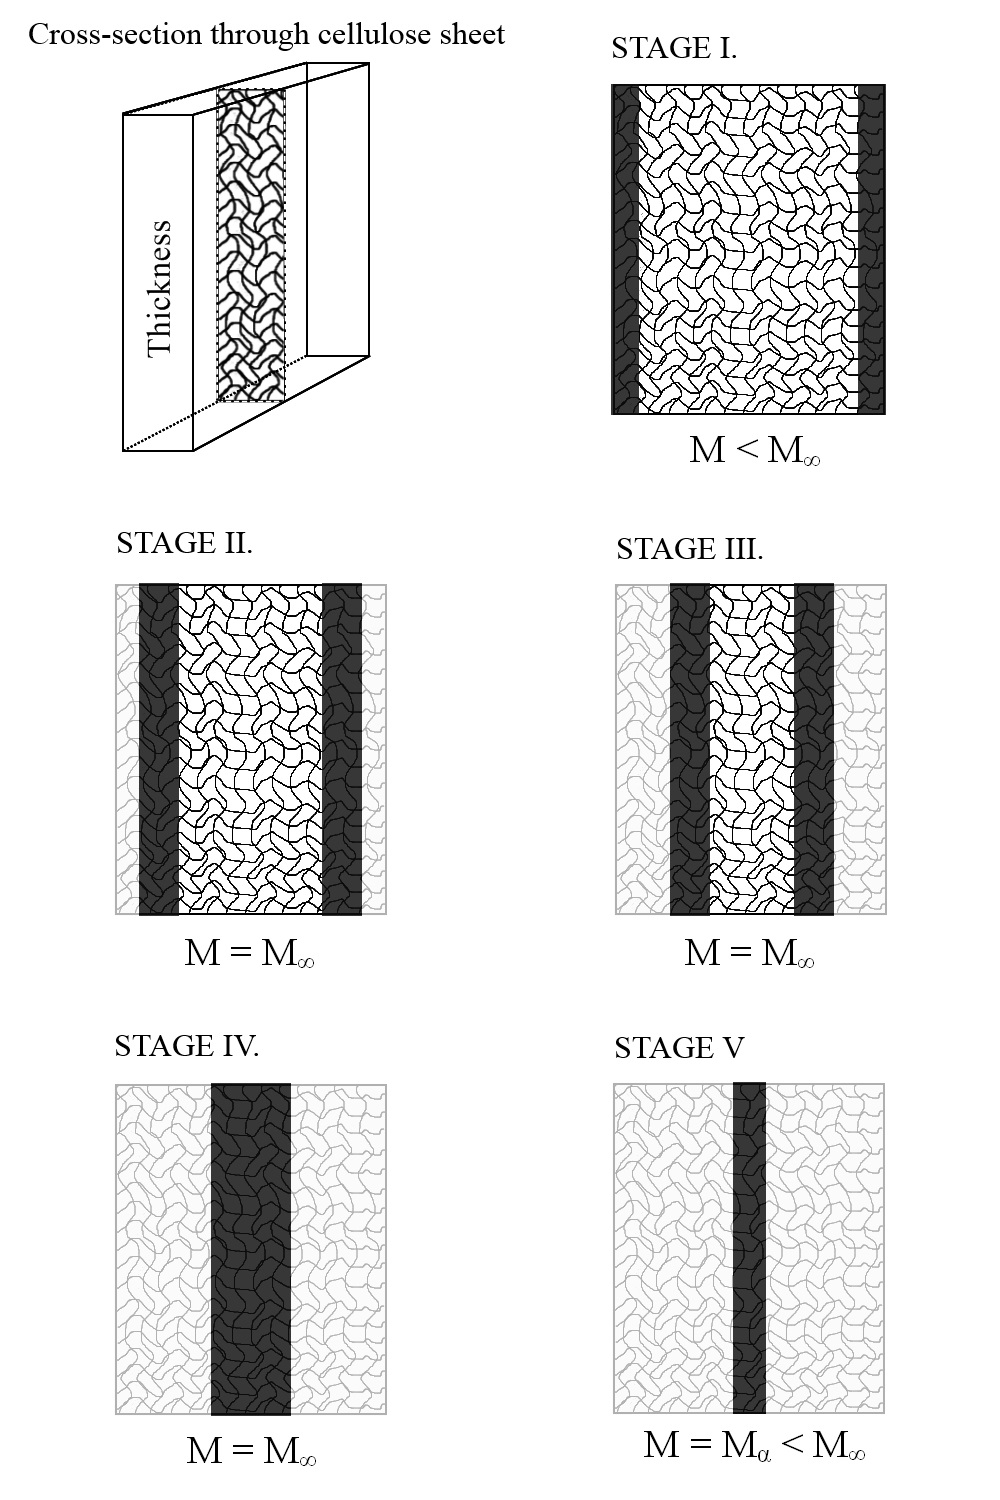
\includegraphics[scale=0.53]{alex_schema.jpg}
  \caption{Conceptual model of cellulolytic biofilm growth and consumption of cellulose sheets. 
    Attachment and growth occurs on both sides of the sheet, individual monolayers form on each fiber and result in a band of active biofilm (i.e., the effective sessile biomass) $M$ (dark band). 
    The ideal carrying capacity, $M_{\infty}$, and the actual carrying capacity, $M_{\alpha}$, are explained in \cite{dumitrache2015mathematicalModeling}.
    Consumed substrate is represented by the light gray areas.
    Figure originally from \cite{dumitrache2015mathematicalModeling}.
  }
  \label{fig:alex_schema}
\end{figure}

A simple mathematical model for cellulolytic biofilm activity and growth on model cellulosic substrate was proposed in \cite{dumitrache2015mathematicalModeling}. 
Here the production of carbon dioxide was used as an indicator of culture metabolism.
Because of this indicator, they focused on overall biofilm performance rather than on detailed biofilm structure.
This led to a reactor-scale model that attributed the spatial effects into logistic-like growth and carrying capacities to limit the bacteria activity in the models.
The model was based on a number of observations on the metabolic activity gathered by online carbon dioxide measurements.
For this model, attention was also put on high-resolution imaging of different stages of biofilm development \citep{dumitrache2013formFunction} and to the physiological behaviour of substrate modification \citep{dumitrache2013tracking}.

The conceptual model of cellulolytic biofilm growth that was followed for their model is shown in Figure \ref{fig:alex_schema}.
This model is based on the relation between \textit{C.thermocellum} growth and cellulose sheet consumption.
The relation is, when \textit{C.thermocellum} grows there exist cellulose sheet consumption, limiting the area of substratum available for bacteria attachment.
Here they express the growth of the biomass in terms of an \textit{ideal} and an \textit{actual} carrying capacity.
The ideal carrying capacity, $M_{\infty}$, refers to the maximum amount of biomass that can be supported when the only limitations are from a deficiency of local space.
This value depends on the properties of the substratum and is assumed to be constant since it is independent of the substrate concentration.
The actual carrying capacity, $M_{\alpha}$, references the amount of biomass that can be supported when the local concentration of substrate mass is limited.
This value is not constant since it is a function of the current substrate concentration.
In essence, \cite{dumitrache2015mathematicalModeling} use the carrying capacity as a means to account for the limitations due to spatial effects.

The model developed by \cite{dumitrache2015mathematicalModeling} followed the five different conceptual growth stages of \textit{C.thermocellum}.
These stages were:
\begin{itemize}
  \item Stage I: Independent colonies of cells grow on the matrix of fibers in the substrate. This occurs initially for all the isolated regions of the biofilm.
  \item Stage II: The biofilm grows inwards. The superficial fibres are consumed and newly unsupported biofilms are released from the cellulose sheet into the aqueous stream.
  \item Stage III: The active biofilm band stabilizes somewhere around the point where superficial fiber deconstruction rate is the equivalent to the inwards penetration rate of the biofilm.
  \item Stage IV: The progression of the biofilm band continues until the remaining amount of usable substrate becomes limited.
  \item Stage V: The remaining cellulose gets consumed without new biofilm being produced. Instead a new generation of non-adherent cells is formed locally.
\end{itemize}
This formulated a system of ordinary differential equation because of the non-diffusivity of the substrate.
These ordinary differential equations resembled traditional growth models in batch cultures more then the typically complex biofilm model seen in studies \citep{wanner2005mathematical}. 

The model developed in \cite{wang2011spatial} focused more on detailing the qualitative aspects of a single \textit{C.thermocellum} colony in terms of spatio-temporal development.  
The reaction kinetics were ignored as they assumed that when bacteria occupied a new space all the substrate would be immediately utilised.
This was completed by use of a nine-neighbour square cellular automata on a $30 \times 15$ grid with a single grid cell as an inoculation point.
The model results matched the experimental results they gathered.
This was the first model to consider the spatial development of \textit{C.thermocellum} at a small scale.
Using cellular automata with such a coarse grid gave them a discrete representation of the system they modelled.
One purpose of this thesis is to extend this concept to a continuous model similar to \cite{eberl2001deterministic} but instead using the assumptions and growth function that match the behaviour of \textit{C.thermocellum}.

There are problems with trying to extend \textit{C.thermocellum} to a spatially considerate continuum model.
Because the substratum used for attachment is consumed with biofilm growth and the stationary nature of the cellulose sheets, this problem becomes significantly different from other biofilm models which are based on the aqueous, free-floating environment where biofilms typically develop.
At the meso-scale, our \textit{C.thermocellum} system must model the development of the biofilm along the non-diffusing individual fibers of the cellulose sheet structure.
Thus, these two categories of biofilm models differ mainly in their consideration of substrate diffusion, with \textit{C.thermocellum} there is none.

Our problem originates from the ordinary differential equation model from \cite{dumitrache2015mathematicalModeling}.
Here we include the double-degenerate parabolic model of biofilm formation from \cite{eberl2001deterministic} for the spatial consideration.
This type of model arises when a volume filling problem has a finite speed of interface propagation \citep{khassehkhan2009nonlinearMaster}.
A density-dependent diffusion model with reaction terms that match with the behaviour of \textit{C.thermocellum} is what is handled here.
The spatial operator for biofilm spreading shows two non-standard diffusion effects:
\begin{itemize} 
  \item A power law degeneracy similar to the porous medium equation for local biomass at the interface of the biofilm \citep{gurtin1977diffusion}.
  \item A singularity in the diffusion coefficient when the biofilm approaches maximum biomass density. 
\end{itemize}
Both of these effects together lead to the development of sharp and steep interfaces in the model solutions that mark the separation of the actual biofilm from its liquid environment.
Such propagating interface problems in partial differential equations often are difficult to treat numerically.

The mathematical models which focus on the growth dynamics of biological films are usually systems of partial differential equations.
%\cite{efendiev2002existencelongtime} showed that models which focus on the growth dynamics of biological films typically are systems of partial differential equations.
These models are built on some of the significant features of biofilm growth observed throughout the practice, such as:
\begin{enumerate}[a)]
  \item the presence of a sharp front of biomass at the solid to fluid transition region,
  \item the existence of a threshold of biomass density,
  \item the spreading of biomass is only notable when local densities approach the threshold of sustainability,
  \item the use of reaction kinetics mechanisms to model the production of biomass,
  \item the compatibility of biomass spreading with nutrient transfer and consumption mechanism models.
\end{enumerate}
There exists mathematical background for these systems of equations that prove existence and uniqueness of positive and bounded solutions.
However, the complexity of these nonlinear partial differential equations have made providing analytical expressions of the solutions practically impossible, when given biologically meaningful initial conditions.

This forces numerical computational approaches to be taken for simulating the growth of these microbial colonies.
Some techniques with the finite-difference method have been used for these problems. 
This approach has been proposed in \cite{eberl2007finite} for deterministic models.

%!% l.195-202 .. This sentence will need to be re-written
In this thesis, the finite-difference method is treated as a semi-implicit numerical method similar to \cite{eberl2007finite}.
Here, the method is extended to use a fixed-point iteration to facilitate the computations of the degeneracy from the biomass diffusion.
This turns the semi-implicit method into a fully-implicit method.
The validity of this method is unknown and put under scrutiny by simulating the \textit{C.thermocellum} system during this thesis.
This system has a partial differential equation for the diffusion-reaction equation of biomass and an ordinary differential equation for the non-diffusing substrate concentrations.

